\documentclass[11pt,a4paper]{article}
\usepackage[margin=18mm]{geometry}
\usepackage{graphicx}
\usepackage{booktabs}
\usepackage{tabularx}
\usepackage{array}
\usepackage{xcolor}
\usepackage{amsmath}
\usepackage{enumitem}
\usepackage{fancyhdr}
\usepackage{hyperref}
\usepackage{listings}
\usepackage{tikz}
\usetikzlibrary{arrows.meta,positioning,shapes.geometric}
\definecolor{navy}{HTML}{17365D}
\definecolor{accent}{HTML}{2F75B5}
\definecolor{soft}{HTML}{EAF2F8}
\definecolor{dark}{HTML}{263238}
\hypersetup{colorlinks=true,linkcolor=navy,urlcolor=accent}
\pagestyle{fancy}
\fancyhf{}
\lhead{MuSHR Vision-Aware Autonomous Racing Challenge}
\rhead{5-Day Intermediate Robotics Assignment}
\cfoot{\thepage}
\setlength{\headheight}{14pt}
\setlist[itemize]{nosep,leftmargin=5mm}
\setlist[enumerate]{nosep,leftmargin=6mm}
\lstset{basicstyle=\ttfamily\small,frame=single,breaklines=true,backgroundcolor=\color{soft},showstringspaces=false}
\newcommand{\deliverable}[1]{\textbf{Deliverable:} #1}
\begin{document}

\begin{titlepage}
\centering
\vspace*{17mm}
{\Huge\bfseries\color{navy} MuSHR Vision-Aware\\[3mm]Autonomous Racing Challenge\par}
\vspace{7mm}
{\Large A Five-Day Simulation-Only Assignment for Intermediate Robotics Students\par}
\vspace{15mm}
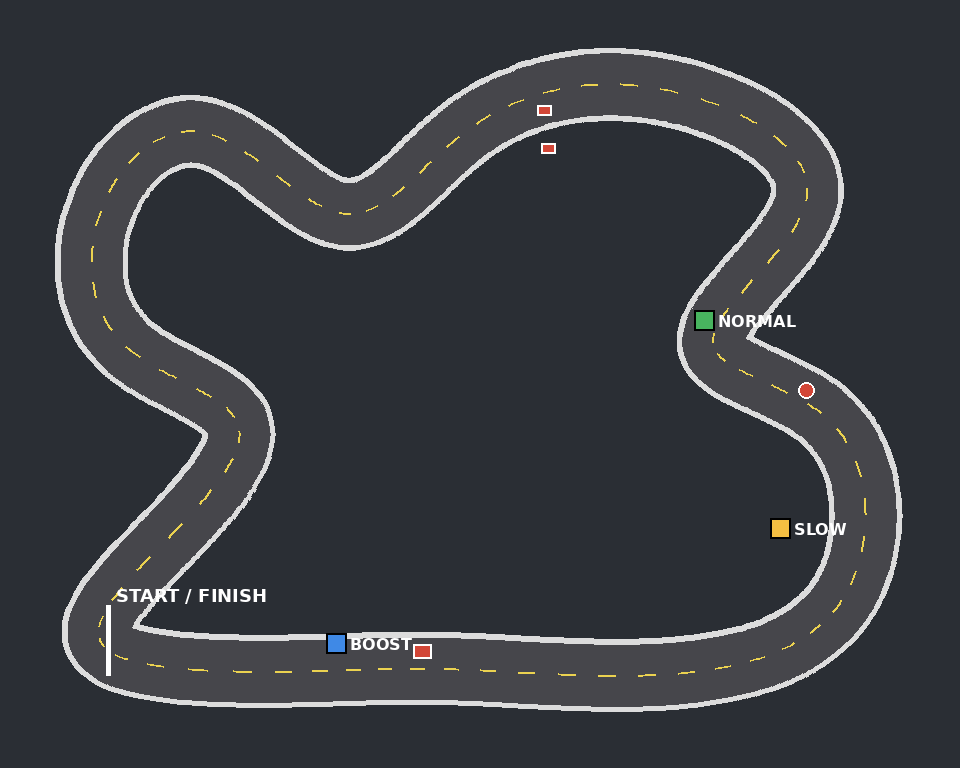
\includegraphics[width=0.92\textwidth]{../track/training_track_preview.png}
\vfill
\begin{tabular}{rl}
Duration: & 5 working days\\
Team size: & 2--4 students\\
Platform: & MuSHR-compatible simulation\\
Primary sensors: & 2D LiDAR, odometry/localization, forward RGB camera\\
Control output: & Ackermann steering and speed commands
\end{tabular}
\vfill
{\small Instructor-provided track, obstacle layouts, centre-line waypoints and visual sign assets are included with this handout.}
\end{titlepage}

\tableofcontents
\newpage

\section{Challenge Overview}
Design an autonomous racing stack that completes three consecutive laps on a known training track and generalizes to an evaluation configuration. The vehicle must race quickly, remain inside the track, avoid static obstacles, interpret visual speed signs and recover from common failures without manual control.

The task is intentionally simulation-only. Mapping and SLAM are outside the scope. Students receive an occupancy-grid map, an initial pose and centre-line waypoints. Their main work is control, local safety, computer vision, integration and quantitative evaluation.

\subsection*{Required capabilities}
\begin{enumerate}
  \item Follow the supplied track without teleoperation.
  \item Increase speed on straights and brake before high-curvature sections.
  \item Use LiDAR to avoid obstacles and prevent unsafe commands.
  \item Detect track-side visual signs from a simulated front camera.
  \item Apply the detected sign as a temporary speed-zone constraint.
  \item Detect being stuck or off-course and execute an automatic recovery.
  \item Complete three consecutive laps and produce reproducible logs.
\end{enumerate}

\section{Learning Outcomes}
By the end of the assignment, students should be able to:
\begin{itemize}
  \item implement and tune a geometric path-following controller;
  \item derive a speed profile from path curvature;
  \item process a \texttt{LaserScan} for emergency braking and local avoidance;
  \item build an OpenCV-based fiducial-marker detector;
  \item combine nominal control and safety constraints;
  \item implement a finite-state recovery controller;
  \item evaluate a robot using lap time, collision rate, sign accuracy and robustness metrics.
\end{itemize}

\section{Provided Simulation Assets}
The assignment package contains:
\begin{itemize}
  \item \texttt{mushr\_training\_track.pgm} and \texttt{.yaml}: ROS-style occupancy grid;
  \item \texttt{centerline\_waypoints.csv}: waypoint ID, $x$, $y$ and heading;
  \item \texttt{obstacle\_sets.yaml}: one public development layout and hidden evaluation layouts;
  \item \texttt{vision\_sign\_layouts.yaml}: public and hidden sign placements;
  \item three ArUco sign-board textures: SLOW, NORMAL and BOOST;
  \item an annotated track preview and named track sectors.
\end{itemize}

\subsection{Track characteristics}
The course occupies approximately $30\,\mathrm{m}\times24\,\mathrm{m}$ and has a nominal width of about $2.3\,\mathrm{m}$. It includes a long straight, fast sweepers, an S-shaped transition, a tighter eastern complex and a western recovery-sensitive section. Solid collision boundaries must be LiDAR-visible; decorative painted lines alone are not sufficient.

\begin{figure}[h]
\centering
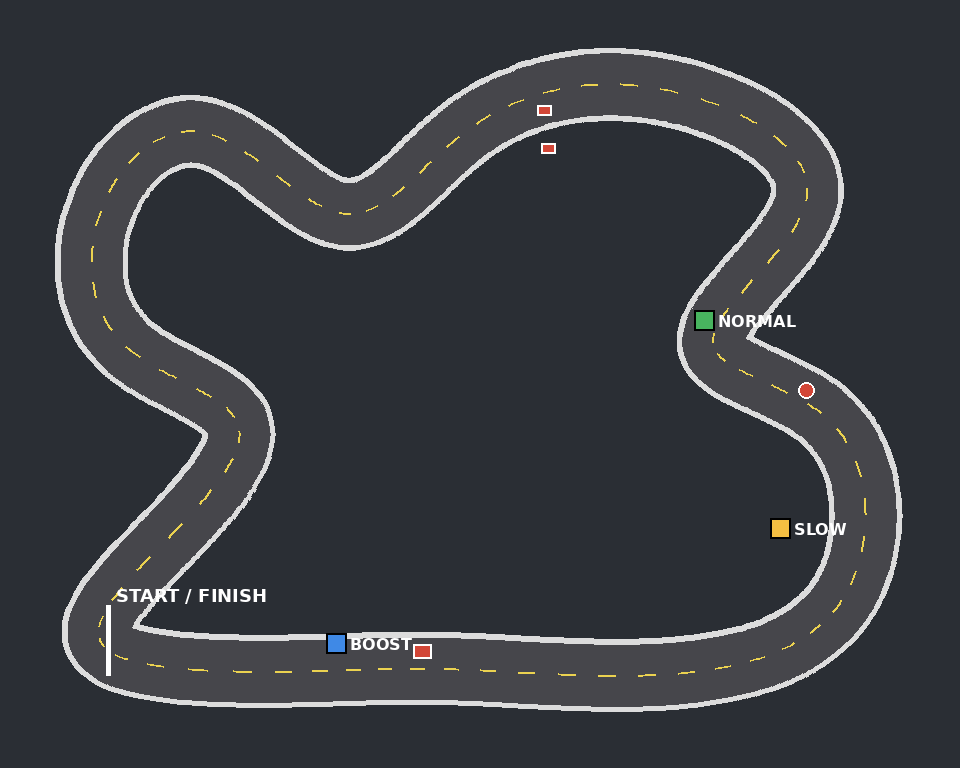
\includegraphics[width=0.95\textwidth]{../track/training_track_preview.png}
\caption{Development track. Red shapes are the public development obstacles. Colored squares indicate public visual-sign locations.}
\end{figure}

\section{Computer-Vision Component}
The vehicle receives images from a simulated forward-facing RGB camera. Track-side boards carry ArUco markers from the OpenCV \texttt{DICT\_4X4\_50} dictionary.

\begin{center}
\begin{tabular}{cccc}
\toprule
Marker ID & Sign & Nominal speed cap & Required response\\
\midrule
10 & SLOW & $1.0\,\mathrm{m/s}$ & Reduce speed before the following complex\\
20 & NORMAL & $1.8\,\mathrm{m/s}$ & Restore the normal race-speed ceiling\\
30 & BOOST & $2.5\,\mathrm{m/s}$ & Permit higher speed where curvature and safety allow\\
\bottomrule
\end{tabular}
\end{center}

The sign value is an \emph{upper bound}, not a direct throttle command. The final speed must also satisfy curvature, acceleration and LiDAR constraints:
\[
v_{\mathrm{cmd}}=\min\left(v_{\mathrm{curve}},v_{\mathrm{sign}},v_{\mathrm{lidar}}\right).
\]

\subsection*{Vision requirements}
\begin{itemize}
  \item Detect marker ID and publish the active speed-zone state.
  \item Reject isolated false detections using temporal confirmation, confidence or repeated frames.
  \item Retain the most recently confirmed sign until a new valid sign is observed.
  \item Log timestamp, marker ID, detection confidence or reprojection measure, and active speed cap.
  \item Demonstrate operation under at least two image perturbations: brightness change, blur, partial occlusion or image noise.
\end{itemize}

Deep learning is not required. A correct OpenCV ArUco pipeline is sufficient and keeps the five-day scope realistic.

\section{Recommended System Architecture}
\begin{center}
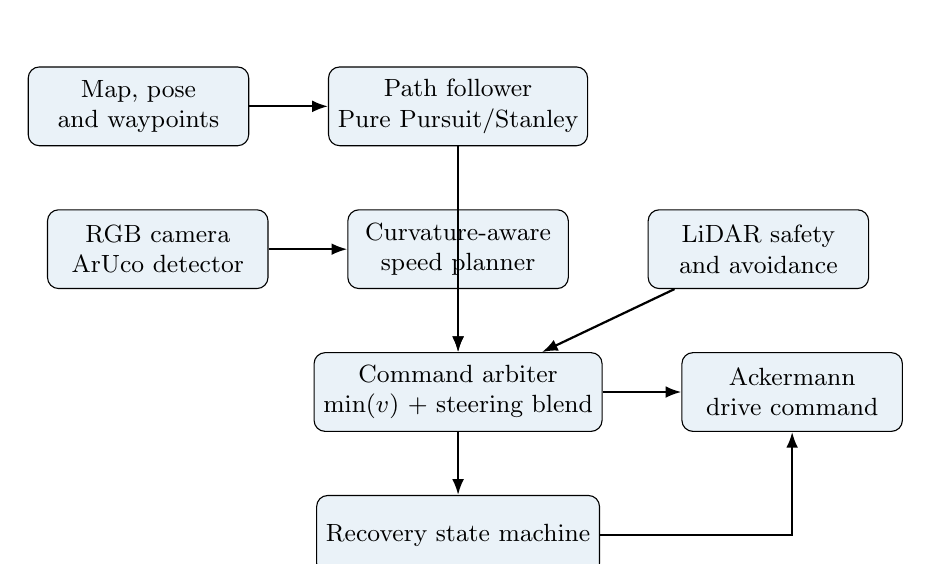
\begin{tikzpicture}[node distance=8mm and 10mm, every node/.style={font=\small}, box/.style={draw,rounded corners,align=center,minimum height=10mm,minimum width=28mm,fill=soft}, arrow/.style={-{Latex[length=2mm]},thick}]
\node[box] (map) {Map, pose\\and waypoints};
\node[box,right=of map] (path) {Path follower\\Pure Pursuit/Stanley};
\node[box,below=of path] (curve) {Curvature-aware\\speed planner};
\node[box,left=of curve] (cam) {RGB camera\\ArUco detector};
\node[box,right=of curve] (lidar) {LiDAR safety\\and avoidance};
\node[box,below=of curve] (arb) {Command arbiter\\$\min(v)$ + steering blend};
\node[box,below=of arb] (fsm) {Recovery state machine};
\node[box,right=of arb] (drive) {Ackermann\\drive command};
\draw[arrow] (map)--(path);
\draw[arrow] (path)--(arb);
\draw[arrow] (curve)--(arb);
\draw[arrow] (cam)--(curve);
\draw[arrow] (lidar)--(arb);
\draw[arrow] (arb)--(drive);
\draw[arrow] (arb)--(fsm);
\draw[arrow] (fsm)-| (drive);
\end{tikzpicture}
\end{center}

A suggested curvature speed law is
\[
v_{\mathrm{curve}}=\mathrm{clip}\left(\frac{v_{\max}}{1+k_{\kappa}|\kappa|},v_{\min},v_{\max}\right).
\]
Use acceleration and deceleration limits to avoid discontinuous commands.

\section{Obstacle Challenge}
Development obstacles are visible in the supplied layout. Evaluation uses a different instructor-selected layout. All layouts leave a feasible passage; no obstacle fully blocks the course.

The controller must:
\begin{itemize}
  \item reduce speed as forward clearance decreases;
  \item trigger an emergency stop below a configured threshold;
  \item steer around partial blockages without crossing the track boundary;
  \item avoid oscillation in narrow passages;
  \item resume nominal racing after the obstacle is cleared.
\end{itemize}

The final evaluation can move obstacles and signs independently. Hard-coded actions tied to waypoint numbers will therefore receive poor robustness marks.

\section{Five-Day Schedule and Checkpoints}
\subsection*{Day 1: Platform, topics and baseline lap}
Inspect the simulator interfaces, teleoperate the vehicle, visualize the map and run a supplied low-speed baseline. Implement waypoint loading and lap counting.

\deliverable{One collision-free low-speed lap, topic/interface diagram and a short baseline log.}

\subsection*{Day 2: Path following}
Implement Pure Pursuit, Stanley or another approved geometric controller. Tune look-ahead and steering limits. Complete three fixed-speed laps.

\deliverable{Controller code, parameter file and plot of lateral/heading error over one lap.}

\subsection*{Day 3: Speed planning and vision}
Estimate upcoming curvature and generate a smooth speed profile. Implement ArUco sign detection and integrate the active sign speed cap.

\deliverable{Three-sign detection demo, sign log, speed-profile plot and a lap showing at least two speed-zone transitions.}

\subsection*{Day 4: LiDAR safety and recovery}
Add obstacle-aware speed limiting, emergency braking, local avoidance, stuck detection and a recovery state machine. Test image perturbations and at least two forced recovery cases.

\deliverable{Obstacle run, recovery-state log, safety-threshold justification and vision robustness table.}

\subsection*{Day 5: Final evaluation and presentation}
Tune only on the public development configuration. Submit the final package before the hidden evaluation configuration is revealed. Each team receives three official runs.

\deliverable{Final repository, report, logs, plots, demonstration video and five-minute presentation.}

\section{Minimum Software Interface}
The instructor should expose an equivalent interface even if exact topic names differ across simulator branches.

\begin{lstlisting}
Inputs
  /scan                     sensor_msgs/LaserScan
  /camera/front/image_raw   sensor_msgs/Image
  /odom or /pose            nav_msgs/Odometry or pose equivalent

Output
  /drive                    ackermann_msgs/AckermannDriveStamped

Recommended team outputs
  /race/active_sign         std_msgs/Int32
  /race/target_speed        std_msgs/Float32
  /race/state               std_msgs/String
  /race/lap_count           std_msgs/Int32
\end{lstlisting}

\section{Rules and Constraints}
\begin{itemize}
  \item No teleoperation after the official run begins.
  \item The supplied centre-line may be smoothed or locally offset, but the map may not be modified.
  \item Hidden obstacle and sign positions must not be read directly from instructor configuration files at runtime.
  \item LiDAR must be used for collision safety; vision alone is insufficient for obstacle avoidance.
  \item Camera images must be processed online during the run.
  \item Pretrained neural networks are optional but provide no automatic bonus.
  \item A manual reset ends the current official run and incurs the reset penalty.
\end{itemize}

\section{Evaluation Protocol}
\subsection*{Round 1: Clean-track time trial}
Three laps, no obstacles, public sign layout. Measures path tracking, speed planning and vision integration.

\subsection*{Round 2: Obstacle race}
Three laps with development-style static obstacles and a changed sign layout. Measures local safety and non-memorized perception.

\subsection*{Round 3: Robustness run}
One or two laps using an instructor-selected evaluation obstacle set, changed sign positions and mild camera perturbation.

\subsection*{Penalties}
\begin{center}
\begin{tabular}{lr}
\toprule
Event & Penalty\\
\midrule
Obstacle contact & +10 s\\
Track-boundary contact & +5 s\\
Missed required sign response & +8 s each\\
False sign transition & +4 s each\\
Manual reset & +20 s and recovery score loss\\
Incomplete lap & Lap not scored\\
\bottomrule
\end{tabular}
\end{center}

\section{Grading Rubric}
\begin{center}
\begin{tabularx}{\textwidth}{Xr}
\toprule
Component & Weight\\
\midrule
Reliable autonomous completion and lap counting & 20\%\\
Path following and curvature-aware speed control & 20\%\\
LiDAR obstacle safety and local avoidance & 18\%\\
Computer-vision sign detection and robustness & 17\%\\
Recovery behaviour and fault handling & 10\%\\
Experimental analysis, plots and reproducibility & 10\%\\
Code quality and presentation & 5\%\\
\bottomrule
\end{tabularx}
\end{center}

To pass, a team must complete at least one autonomous lap, detect at least two marker classes online, and demonstrate an emergency stop. Racing speed cannot compensate for failure of these minimum safety and perception requirements.

\section{Required Submission}
Submit one compressed archive or repository containing:
\begin{enumerate}
  \item ROS package(s), launch files and configuration files;
  \item a README with installation and exact run commands;
  \item a one-page architecture diagram;
  \item controller, vision and recovery parameter files;
  \item CSV logs for time, pose, speed, steering, minimum LiDAR range, active sign and state;
  \item plots of lap speed, steering, tracking error and obstacle clearance;
  \item a vision evaluation table with precision, recall or detection success rate;
  \item a two-to-three-minute demonstration video;
  \item a report of at most five pages excluding appendices;
  \item a brief statement of each team member's contribution.
\end{enumerate}

\section{Suggested Report Questions}
\begin{enumerate}
  \item How was look-ahead distance selected, and should it vary with speed?
  \item How was curvature estimated from discrete waypoints?
  \item Which constraint most often limited speed: curvature, sign or LiDAR?
  \item How did the marker detector reject false positives and duplicate observations?
  \item What failure modes remained on the hidden configuration?
  \item Which single change would most improve lap time without reducing safety?
\end{enumerate}

\section{Instructor Notes}
The included map is a standard ROS-style occupancy grid rather than a simulator-specific world file. The exact MuSHR simulator branch may require a thin adapter for map loading, obstacle spawning, RGB camera publication and topic names. Provide students a tested launch command and baseline controller before Day 1. Keep evaluation layouts private and verify every generated obstacle set leaves a physically feasible route.

The vision task is deliberately fiducial-based. It teaches image transport, camera geometry, online detection, filtering and decision integration without requiring dataset collection or GPU training. For a more advanced cohort, replace one marker class with a conventional colored or symbolic sign and require a classical contour/classification pipeline.

\section{References}
\begin{enumerate}
  \item S. S. Srinivasa et al., ``MuSHR: A Low-Cost, Open-Source Robotic Racecar for Education and Research,'' 2019.
  \item MuSHR project repository, Personal Robotics Lab, University of Washington: \url{https://github.com/prl-mushr/mushr}.
  \item OpenCV documentation, ArUco marker detection module: \url{https://docs.opencv.org/4.x/d5/dae/tutorial_aruco_detection.html}.
\end{enumerate}

\end{document}
